Robots need to be able to connect language to their environment in order to discuss real world objects with humans.
Mapping from referring expressions such as ``the blue cup'' to an object referent in the world is an example of the \textit{symbol grounding problem}~\cite{harnad:phys90}.
Symbol grounding involves connecting internal representations of information in a machine to real world data from its sensory perception.
\textit{Grounded language learning} bridges these symbols with natural language.

Early work on grounded language learning enabled a machine to map from adjectives and nouns such as ``red'' and ``block'' to objects in a scene through vision-based classifiers~\cite{roy:evocomm01}.
We refer to adjectives and nouns that describe properties of objects as language \textit{predicates}.
Most work has focused on grounding predicates through visual information. However, other sensory modalities such as haptic and auditory are also useful in allowing robots to discriminate between object categories~\cite{sinapov:icra14}.
This paper explores grounding language predicates by considering visual, haptic, auditory, and proprioceptive senses. 

A home or office robot can explore objects in an unsupervised way to gather perceptual data, but needs human supervision to connect this data to language.
Learning grounded semantics through human-robot dialog allows a system to acquire the relevant knowledge without the need for laborious labeling of numerous objects for every potential lexical descriptor.
A few groups have explored learning from interactive linguistic games such as \ispy and ``20 Questions'' \cite{parde:ijcai15,vogel:aaai10}; however, these studies only employed vision (see Section \ref{sec:relatedwork}).

\begin{figure}
\centering
\begin{tabular}{cc}
	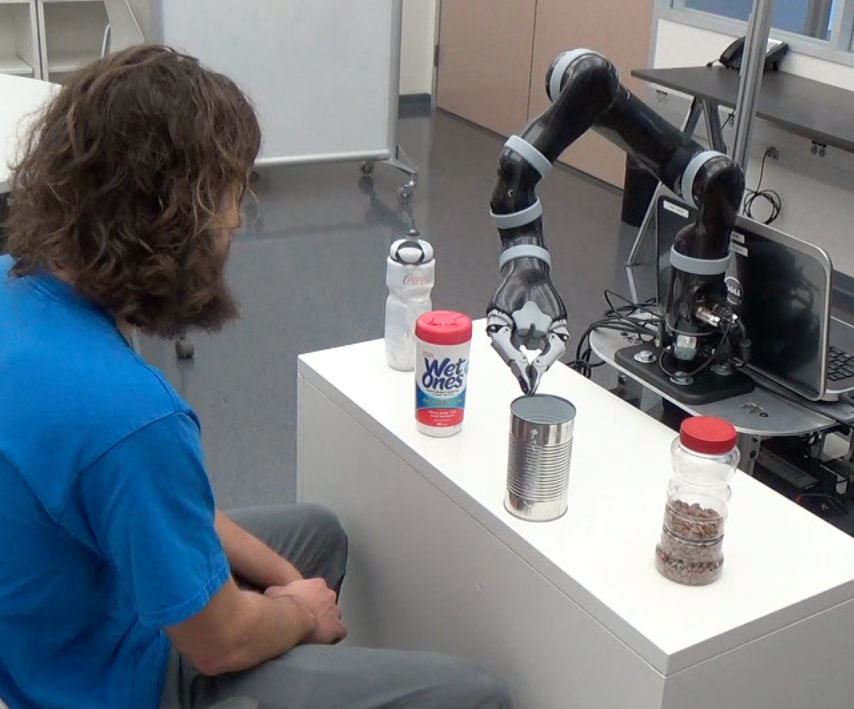
\includegraphics[width=0.225\textwidth]{figures/silver_round_and_empty_cropped.png} &
	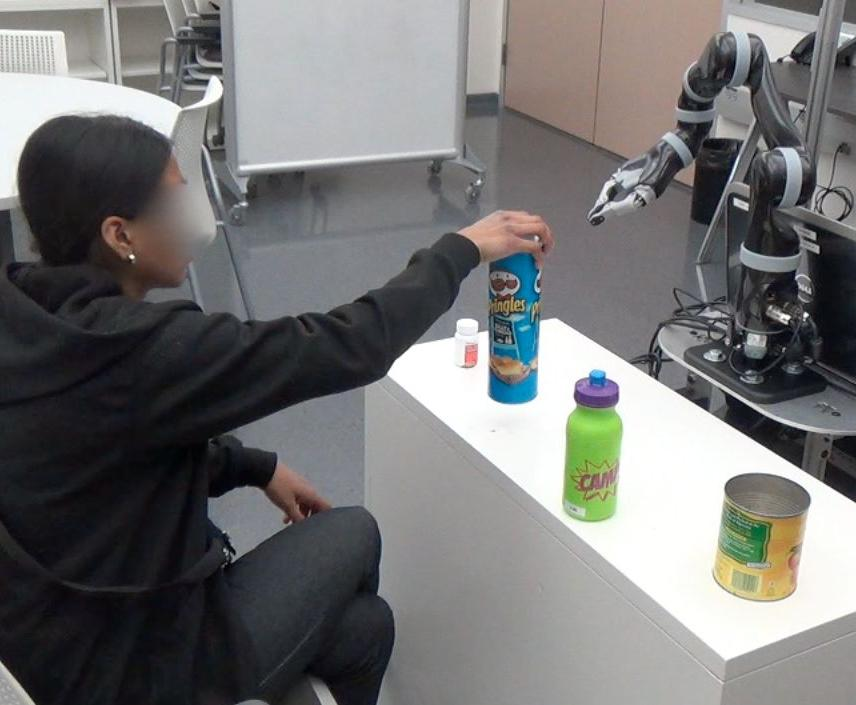
\includegraphics[width=0.225\textwidth]{figures/light_tall_tub_cropped.jpg} \\
\end{tabular}
\caption{\textbf{Left}: the robot guesses an object described by a human participant as ``silver, round, and empty.'' \textbf{Right}: a human participant guesses an object described by the robot as ``light,'' ``tall,'' and ``tub.''}
\label{fig:ispy}
\end{figure}

We use a variation on the children's game \ispy as a learning framework for gathering human language labels for objects to learn multi-modal grounded lexical semantics (Figure~\ref{fig:ispy}).
Our experimental results test generalization to new objects not seen during training and illustrate both that the system learns accurate word meanings and that modalities beyond vision improve its performance.

To our knowledge, this is the first robotic system to perform natural language grounding using multi-modal sensory perception through feedback with human users.